\documentclass{article}

% NeurIPS 2026 submission mode is anonymous and includes line numbers.
% For a non-anonymous local draft, change the next line to:
% \usepackage[preprint]{neurips_2026}
\PassOptionsToPackage{numbers,sort&compress}{natbib}
\usepackage{neurips_2026}

\usepackage[utf8]{inputenc}
\usepackage[T1]{fontenc}
\usepackage{hyperref}
\usepackage{url}
\usepackage{booktabs}
\usepackage{amsfonts}
\usepackage{amsmath}
\usepackage{nicefrac}
\usepackage{microtype}
\usepackage{xcolor}
\usepackage{graphicx}
\usepackage{subcaption}
\usepackage{algorithm}
\usepackage{algorithmic}
\usepackage{multirow}
\usepackage{float}

% Custom colors for consistency
\definecolor{cacheblue}{HTML}{2C5282}
\definecolor{loadred}{HTML}{C53030}
\definecolor{accentgreen}{HTML}{276749}

\title{Cache-Aware Gateway Routing for Multi-Instance LLM Serving:\\A Systematic Evaluation of Locality vs.\ Load Balance Tradeoffs}

\author{
  David Mike-Ewewie \\
  Department of Computer Science and Electrical Engineering \\
  University of Texas Permian Basin \\
  \texttt{email omitted for public repository} \\
}

\begin{document}

\maketitle

% ===========================================================================
% ABSTRACT
% ===========================================================================
\begin{abstract}
Large language model (LLM) serving deployments run multiple inference engine instances behind a load balancer, where each instance maintains its own KV cache of previously computed attention states. Routing a request to an instance that already holds relevant cached prefixes can reduce time-to-first-token (TTFT), yet aggressive cache affinity can also concentrate traffic and increase queueing delay. We present an empirical evaluation of six gateway-level routing policies---three load-only baselines (round-robin, join-shortest-queue, power-of-two-choices) and three cache-aware policies (session affinity, prefix-key affinity, and a tunable load+cache-aware scoring function)---for multi-instance vLLM serving with prefix caching enabled. Using vLLM's native Prometheus metrics, we measure TTFT, prefix-cache hit rate, client-observed latency, and load imbalance on ShareGPT multi-turn and synthetic RAG workloads. The results are mixed in a useful way: cache-aware policies improve locality on multi-turn conversations, but RAG workloads with a single shared system prompt can saturate prefix-cache hit rate across all policies, making load imbalance the decisive metric. In particular, a cache-heavy scoring policy can collapse all RAG traffic onto one backend, while balanced $\alpha/\beta$ settings preserve locality with substantially better load distribution. Our two-instance prototype shares a single GPU; all latency comparisons are therefore \emph{relative}, with every policy exposed to the same contention. We release the router implementation, experiment runner, and generated analysis artifacts for reproducibility.
\end{abstract}

% ===========================================================================
% 1. INTRODUCTION
% ===========================================================================
\section{Introduction}
\label{sec:intro}

Deploying large language models (LLMs) at scale requires running multiple inference engine instances to meet throughput demands, provide fault isolation, and accommodate models that exceed single-device memory~\citep{kwon2023pagedattention, zhong2024distserve}. In such multi-instance deployments, a gateway (load balancer) sits in front of the instances and routes each incoming request to one of them.

Modern LLM inference engines such as vLLM~\citep{kwon2023pagedattention} and SGLang~\citep{zheng2024sglang} implement \emph{prefix caching}---reusing previously computed KV cache entries when a new request shares a prefix with an earlier one. Prefix caching can dramatically reduce the prefill phase duration, which dominates time-to-first-token (TTFT) for long-context requests. However, KV caches are \emph{per-instance}: if a gateway naively distributes requests across instances, the same prefix may be recomputed on every instance, wasting the locality that prefix caching provides.

This creates a fundamental tension. \textbf{Cache-aware routing} steers requests toward instances that likely hold relevant cached prefixes, improving cache reuse. But concentrating requests on specific instances can create \textbf{load imbalance}---some instances become overloaded while others idle, increasing tail latency through queueing delays.

Recent systems such as Preble~\citep{tao2024preble}, DualMap~\citep{zhu2025dualmap}, and Mooncake~\citep{qin2025mooncake} have demonstrated the value of cache-aware scheduling. However, these systems embed routing logic tightly within custom schedulers or require engine-level modifications, making it difficult to isolate the routing decision from other optimizations and to deploy on unmodified serving backends.

We study a simpler, more practical question: \emph{what routing policy should a gateway use in front of unmodified vLLM instances?} We make three contributions:

\begin{enumerate}
    \item A \textbf{reproducible, apples-to-apples evaluation} of six gateway-level routing policies for vanilla multi-instance vLLM, using vLLM's native metrics for ground-truth TTFT and cache reuse measurements.
    \item A \textbf{proxy-side cache directory} that infers cache state from routing history without engine modification, enabling cache-aware routing at the gateway level.
    \item A \textbf{simple, tunable scoring policy} ($\alpha/\beta$ weighting) plus a sensitivity study showing where cache affinity helps, where it collapses load balance, and which settings are robust under the tested workloads.
\end{enumerate}

This paper reports completed results for the ShareGPT policy comparison, the synthetic RAG policy comparison, and the $\alpha/\beta$ sensitivity sweep.

% ===========================================================================
% 2. BACKGROUND & MOTIVATION
% ===========================================================================
\section{Background and motivation}
\label{sec:background}

\paragraph{KV cache in transformer attention.}
In autoregressive transformer models, each attention layer computes key and value projections for every input token. During generation, previously computed key-value pairs are stored in the \emph{KV cache} to avoid redundant recomputation. For a prefill of $n$ tokens, the attention computation has complexity $O(n^2 \cdot d)$, making long prefixes expensive~\citep{kwon2023pagedattention}.

\paragraph{Prefix caching.}
When two requests share an initial prefix (e.g., the same system prompt), the KV cache entries for that prefix are identical. vLLM's Automatic Prefix Caching (APC)~\citep{kwon2023pagedattention} and SGLang's RadixAttention~\citep{zheng2024sglang} exploit this by matching incoming request prefixes against cached entries, skipping prefill computation for matched tokens. The latency benefit is substantial: a cache hit on a 2K-token prefix can save 50--200\,ms of redundant prefill computation.

\paragraph{Multi-instance serving.}
A single GPU's memory limits the model size and batch capacity of one inference instance. Production deployments therefore run $N \geq 2$ instances, each with its own KV cache. The gateway must choose one instance per request. This is the \emph{routing problem} we study.

\paragraph{The cache--load tradeoff.}
Consider a workload with $K$ distinct system prompts, each used by multiple users. If all requests sharing prompt $k$ are routed to instance $i_k$, that instance caches the prompt once and serves all subsequent requests with a cache hit---maximizing locality. But if prompt $k$ is popular, instance $i_k$ becomes overloaded, increasing queueing delay. The optimal routing balances cache affinity (locality) and load pressure (fairness).

\paragraph{Motivating example.}
In our experimental setup with two vLLM instances (Section~\ref{sec:setup}), round-robin routing achieves a 68\% aggregate cache hit rate across instances. Simply routing all turns of each multi-turn conversation to the same instance (session affinity) raises the cache hit rate to 98.5\%---a 30 percentage-point improvement---but increases load imbalance from 1.0$\times$ to 1.48$\times$, creating hot spots that affect tail latency.

% ===========================================================================
% 3. SYSTEM DESIGN
% ===========================================================================
\section{Routing policy design}
\label{sec:design}

\subsection{System architecture}

We implement our router as a LangGraph-based agentic pipeline that sits in front of $N$ vLLM instances (Figure~\ref{fig:architecture}). Each incoming OpenAI-compatible \texttt{POST /v1/chat/completions} request flows through five stages:

\begin{enumerate}
    \item \textbf{Scrape Metrics}: Poll each instance's Prometheus \texttt{/metrics} endpoint for queue depth, cache hit rate, and TTFT statistics.
    \item \textbf{Update Cache Directory}: Look up cache affinity scores based on routing history.
    \item \textbf{Score and Route}: Run the active routing policy to select a target instance.
    \item \textbf{Forward Request}: Proxy the request to the chosen vLLM backend.
    \item \textbf{Record Results}: Log the outcome and update the cache directory.
\end{enumerate}

\begin{figure}[H]
    \centering
    
\includegraphics[width=0.95\linewidth]{figures/system_architecture.png}
    \caption{System architecture. A FastAPI routing gateway receives OpenAI-compatible chat-completion requests, scrapes vLLM metrics, scores instances using the active policy, forwards the request, and updates a proxy-side cache directory. Each vLLM instance maintains its own KV cache with prefix caching enabled.}
    \label{fig:architecture}
\end{figure}

\subsection{Routing policies}

We evaluate six policies organized into two categories:

\paragraph{Load-only baselines} make routing decisions using only queue depth information, ignoring cache state entirely.

\begin{itemize}
    \item \textbf{Round-Robin (RR)}: Cycle through instances sequentially. This is the simplest possible policy with zero intelligence.
    \item \textbf{Join-Shortest-Queue (JSQ)}: Route to the instance with the fewest waiting requests. Ties are broken randomly to avoid hot-spotting.
    \item \textbf{Power-of-Two-Choices (P2C)}: Sample two random instances and pick the one with the shorter queue. This achieves exponential improvement in tail behavior over random assignment~\citep{mitzenmacher2001power}.
\end{itemize}

\paragraph{Cache-aware policies} incorporate cache state information into routing decisions, potentially sacrificing some load balance for improved cache locality.

\begin{itemize}
    \item \textbf{Session Affinity Hash (SA)}: Hash the session or user ID to a fixed instance using a deterministic hash function. All turns of a multi-turn conversation go to the same instance, maximizing per-session prefix reuse.
    \item \textbf{Prefix-Key Affinity (PK)}: Hash the first 200 characters of the system prompt (or first user message) to an instance, capturing \emph{cross-user} shared prefix locality. If the target instance's queue depth exceeds a threshold $\tau = 10$, fall back to JSQ.
    \item \textbf{Load+Cache-Aware Scoring (LCA)}: Our primary contribution. For each instance $i$, compute a score:
    \begin{equation}
    \label{eq:scoring}
    s_i = \alpha \cdot \textit{cache\_affinity}_i - \beta \cdot \textit{load\_pressure}_i
    \end{equation}
    where $\textit{cache\_affinity}_i \in [0, 1]$ reflects routing history (1.0 if instance $i$ last received this prefix, 0.5 for session match, 0.0 otherwise). The implementation defines load as waiting requests plus running requests plus router-side in-flight requests, then normalizes by the maximum observed load across instances. Route to $\arg\max_i s_i$, with random tie-breaking. The parameters $\alpha$ and $\beta$ control the cache--load tradeoff.
\end{itemize}

\subsection{Proxy-side cache directory}

Cache-aware routing requires knowing which prefixes are cached on each instance. Querying vLLM's internal cache state is complex and requires engine modification. Instead, we adopt a \emph{proxy-side tracking} approach (``Option C'' in our design space): when we route a request with prefix $P$ to instance $i$, we record the mapping $P \mapsto i$ in an in-memory directory. On subsequent requests with the same prefix, the directory provides cache affinity scores.

This approach has several advantages: (1) \emph{no engine modification}---it works with any vLLM installation out of the box; (2) \emph{low overhead}---a dictionary lookup per request; (3) \emph{reasonable accuracy}---unless cache eviction has occurred, the tracked state reflects reality.

The directory supports a configurable \emph{staleness parameter} $\delta$: entries older than $\delta$ seconds are treated as expired. Setting $\delta = 0$ (no expiration) assumes cached prefixes persist indefinitely; larger values model cache eviction.

% ===========================================================================
% 4. EXPERIMENTAL SETUP
% ===========================================================================
\section{Experimental setup}
\label{sec:setup}

\paragraph{Hardware.} We use a single NVIDIA RTX~5080 GPU with 16\,GB VRAM. Two vLLM instances share this GPU, each allocated 45\% of GPU memory utilization (\texttt{--gpu-memory-utilization 0.45}). Both instances have prefix caching enabled (\texttt{--enable-prefix-caching}).

\begin{quote}
\emph{Caveat}: Both instances share one GPU, introducing contention absent in production multi-GPU deployments. We therefore focus on \textbf{relative} comparisons between policies---all experience the same contention---rather than reporting absolute throughput numbers.
\end{quote}

\paragraph{Model.} We serve Qwen2.5-0.5B-Instruct~\citep{qwen2025} via vLLM. While smaller than production models, Qwen2.5-0.5B produces meaningful compute during prefill and exercises vLLM's prefix caching mechanism identically to larger models, making it suitable for comparative policy evaluation on constrained hardware.

\paragraph{Workloads.}

\begin{itemize}
    \item \textbf{ShareGPT Multi-Turn}: 50 real multi-turn conversations from the ShareGPT dataset, filtered to 2--20 turns. Each human turn is sent as a request with the growing message history, naturally creating prefix-sharing opportunities across turns of the same conversation. This exercises \emph{within-session} prefix reuse.
    \item \textbf{Synthetic RAG}: 100 requests with a fixed long system prompt and varying user queries from different users. This exercises \emph{cross-user} shared-prefix locality---all users share the same system prompt, but have different queries.
\end{itemize}

\paragraph{Metrics.} We collect ground-truth metrics directly from vLLM's Prometheus \texttt{/metrics} endpoint, ensuring measurement fidelity:
\begin{itemize}
    \item \textbf{TTFT}: \texttt{vllm:time\_to\_first\_token\_seconds} (sum and count for mean calculation)
    \item \textbf{Cache hit rate}: $\texttt{prefix\_cache\_hits\_total} \,/\, \texttt{prefix\_cache\_queries\_total}$
    \item \textbf{Queue depth}: \texttt{vllm:num\_requests\_waiting} and \texttt{vllm:num\_requests\_running}
    \item \textbf{Client latency}: End-to-end wall-clock time observed by the experiment runner through the gateway
    \item \textbf{Backend-forward latency}: Time spent by the gateway forwarding the selected request to the chosen backend
\end{itemize}

We compute metric deltas between before/after snapshots to isolate each trial's contribution from cumulative counters.

\paragraph{Methodology.} Each experiment run consists of: (1) a warm-up phase to populate caches, (2) a metrics snapshot, (3) the measurement phase with open-loop load generation at 5\,req/s, and (4) a post-measurement snapshot. We run 3 trials per policy for the policy-comparison experiments with fixed random seeds (42, 123, 7) for reproducibility. Load is generated using Python \texttt{asyncio} with a concurrency limit of 20 to create realistic queue pressure. For the RAG and sensitivity experiments, prompts are namespaced per policy/trial to avoid cross-policy prefix-cache carryover inside the persistent vLLM backends.

\paragraph{Load imbalance ratio.} We define load imbalance as $\rho = n_{\max} / n_{\min}$, where $n_{\max}$ and $n_{\min}$ are the request counts for the most- and least-loaded instances, respectively. Perfect balance yields $\rho = 1.0$.

% ===========================================================================
% 5. EVALUATION
% ===========================================================================
\section{Evaluation}
\label{sec:eval}

This paper reports three completed experiments: a ShareGPT multi-turn policy comparison, a synthetic RAG policy comparison, and an $\alpha/\beta$ sensitivity sweep for the LCA policy. Across all results, the shared-GPU caveat is central: absolute latencies include contention between two vLLM instances on one RTX~5080, so the evidence supports relative comparisons and qualitative tradeoff analysis rather than production-throughput claims.

\subsection{Experiment 1: policy comparison on multi-turn chat}
\label{sec:eval_sharegpt}

Table~\ref{tab:exp1} presents the main results from Experiment~1, averaging across 3 trials per policy. We evaluate all six policies on the ShareGPT multi-turn workload with approximately 150 requests per trial.

\begin{table}[H]
    \caption{Policy comparison on ShareGPT multi-turn chat workload (mean $\pm$ std across 3 trials). Cache hit rate and load imbalance are measured from vLLM Prometheus metrics. \textbf{Bold} indicates best in category.}
    \label{tab:exp1}
    \centering
    \small
    \resizebox{\linewidth}{!}{%
    \begin{tabular}{@{}llcccc@{}}
        \toprule
        \textbf{Type} & \textbf{Policy} & \textbf{vLLM TTFT (ms)} & \textbf{Cache Hit (\%)} & \textbf{Load Imbal.} & \textbf{P95 Lat. (ms)} \\
        \midrule
        \multirow{3}{*}{Load-only}
        & Round-Robin     & $803.7 \pm 196$  & $67.9 \pm 2.0$ & $\mathbf{1.00}$ & $3074$ \\
        & JSQ             & $784.5 \pm 53$   & $94.1 \pm 0.2$ & $1.05$          & $3121$ \\
        & P2C             & $905.6 \pm 149$  & $97.4 \pm 0.7$ & $1.15$          & $3133$ \\
        \midrule
        \multirow{3}{*}{Cache-aware}
        & Session Affin.  & $862.4 \pm 84$   & $\mathbf{98.5} \pm 0.3$ & $1.48$   & $3103$ \\
        & Prefix-Key Aff. & $823.8 \pm 53$   & $98.4 \pm 0.1$ & $1.36$          & $3119$ \\
        & Load+Cache (LCA) & $986.8 \pm 145$ & $98.3 \pm 0.8$ & $\mathbf{1.21}$ & $3221$ \\
        \bottomrule
    \end{tabular}
    }
\end{table}

\paragraph{Key findings.}

\textbf{F1: Cache-aware routing dramatically improves cache hit rates.} Cache-aware policies achieve 98.3--98.5\% cache hit rates compared to 67.9\% for round-robin---a 30 percentage-point improvement. This confirms that gateway-level routing decisions strongly influence whether per-instance prefix caches are effectively utilized.

\textbf{F2: JSQ achieves surprisingly high cache hit rates.} Join-shortest-queue, a purely load-based policy, achieves 94.1\% cache hit rate. This occurs because JSQ tends to route consecutive requests to the same instance when one instance is busy processing the previous request. While not designed for cache affinity, JSQ's ``stay with the idle instance'' behavior provides incidental locality.

\textbf{F3: Pure affinity creates load imbalance.} Session affinity achieves the highest cache hit rate (98.5\%) but also the worst load imbalance (1.48$\times$), meaning one instance receives 48\% more requests than the other. This occurs because conversation lengths vary---some sessions generate many more requests than others, and the hash-based assignment cannot adapt.

\textbf{F4: LCA balances the tradeoff.} The Load+Cache-Aware scoring policy achieves 98.3\% cache hit rate (matching other cache-aware policies) while maintaining the best load balance among cache-aware policies (1.21$\times$ vs.\ 1.48$\times$ for session affinity and 1.36$\times$ for prefix-key affinity). The $\beta \cdot \textit{load\_pressure}$ term actively steers requests away from overloaded instances.

\textbf{F5: P95 tail latency is similar across policies.} All policies exhibit P95 latencies of approximately 3.1\,s, reflecting the shared-GPU contention that dominates tail behavior. The routing policy affects \emph{average} TTFT (through cache hit rates) more than tails, which are bounded by GPU contention.

\paragraph{Per-instance analysis.}
The per-instance breakdown reveals an interesting asymmetry. Under round-robin, instance~0 achieves 98.8\% cache hit rate while instance~1 achieves only 41.9\%. This occurs because ShareGPT conversations have correlated turns---round-robin alternates these between instances, but the warm-up phase loads instance~0's cache first. Cache-aware policies eliminate this asymmetry by consistently routing related requests together.

\subsection{Experiment 2: RAG policy comparison}
\label{sec:eval_rag}

Experiment~2 uses a synthetic RAG workload with one shared system prompt and varied user queries. This setup strongly favors prefix caching: once the shared prompt is warmed, all policies can achieve high prefix-cache hit rates. The result is useful because it separates \emph{cache availability} from \emph{routing stability}. Table~\ref{tab:exp2} shows that every policy reaches roughly 96.8\% cache hit rate, but their load distributions differ sharply.

\begin{table}[H]
    \caption{Experiment~2 RAG policy comparison (mean $\pm$ std across 3 trials). The common system prompt saturates cache hit rate across policies, so load imbalance is the critical differentiator.}
    \label{tab:exp2}
    \centering
    \small
    \resizebox{\linewidth}{!}{%
    \begin{tabular}{@{}lccccc@{}}
        \toprule
        \textbf{Policy} & \textbf{P50 Lat. (ms)} & \textbf{P95 Lat. (ms)} & \textbf{vLLM TTFT (ms)} & \textbf{Cache Hit (\%)} & \textbf{Imbalance} \\
        \midrule
        Round-Robin      & $1404.8 \pm 124.9$ & $2802.9 \pm 169.1$ & $399.6 \pm 14.8$  & $96.8 \pm 0.0$ & $1.00 \pm 0.00$ \\
        JSQ              & $1341.5 \pm 23.2$  & $3548.7 \pm 560.3$ & $383.8 \pm 96.2$  & $96.8 \pm 0.0$ & $1.24 \pm 0.15$ \\
        P2C              & $1380.9 \pm 88.8$  & $3031.0 \pm 106.5$ & $395.5 \pm 121.0$ & $96.8 \pm 0.0$ & $1.19 \pm 0.07$ \\
        Session Affinity & $1315.1 \pm 32.2$  & $3512.4 \pm 585.6$ & $389.6 \pm 66.0$  & $96.8 \pm 0.0$ & $1.92 \pm 0.18$ \\
        Prefix Affinity  & $1073.3 \pm 69.7$  & $2916.7 \pm 194.9$ & $177.5 \pm 31.3$  & $96.8 \pm 0.0$ & $10.11 \pm 2.41$ \\
        LCA              & $965.9 \pm 66.3$   & $2743.5 \pm 793.8$ & $13.9 \pm 0.3$    & $96.8 \pm 0.0$ & $100.00 \pm 0.00$ \\
        \bottomrule
    \end{tabular}}
\end{table}

\begin{figure}[H]
    \centering
    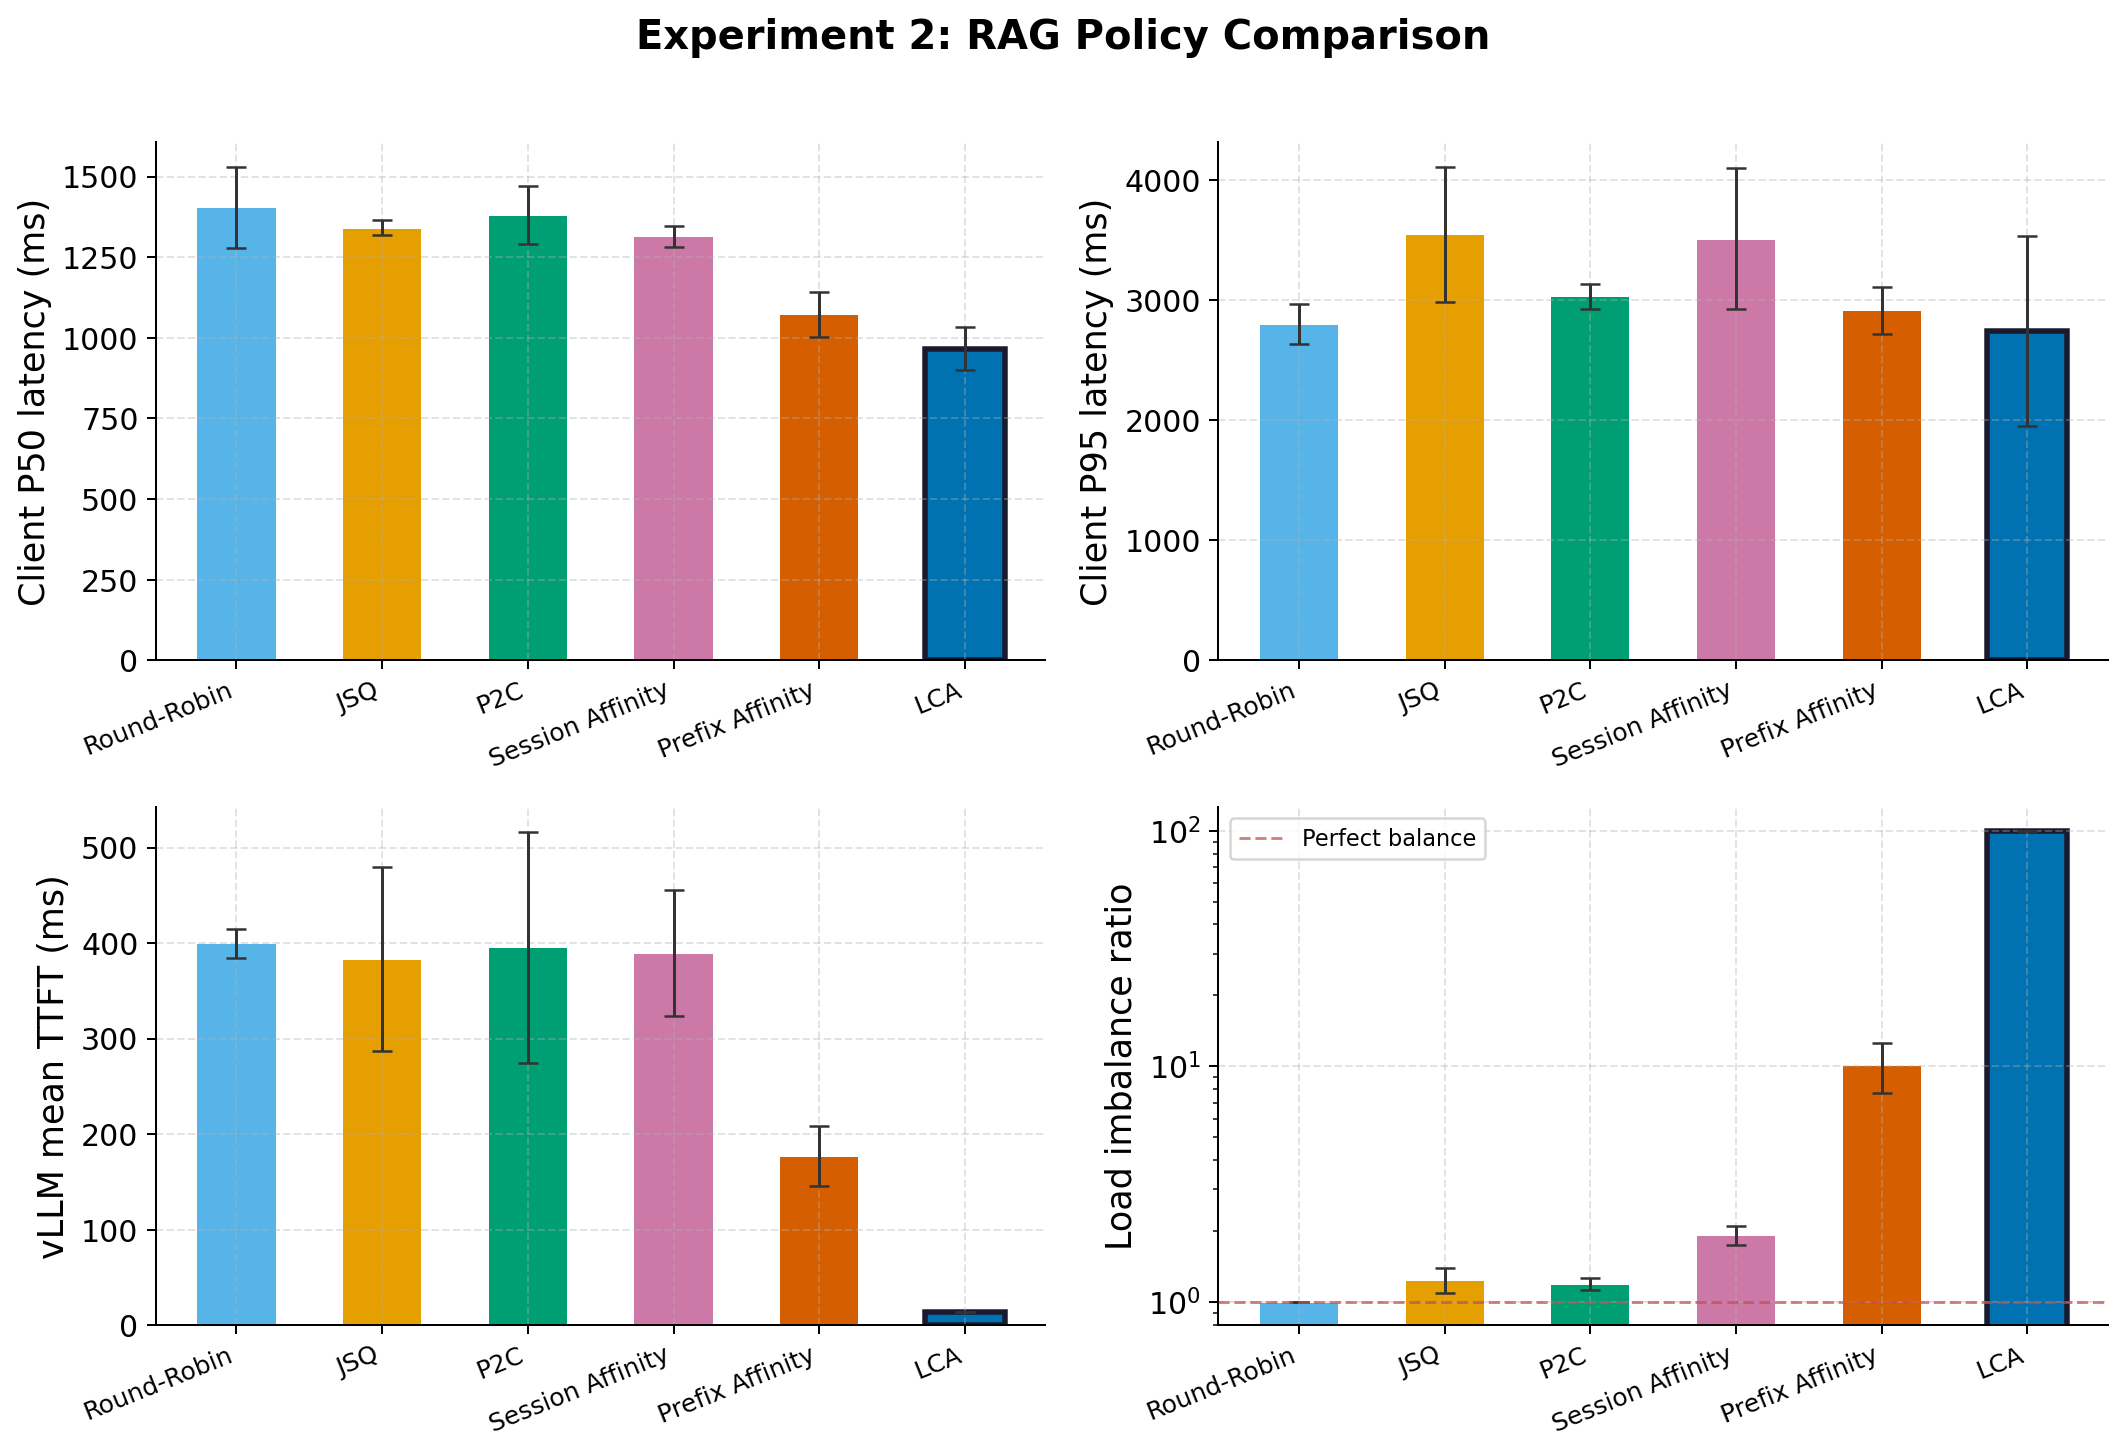
\includegraphics[width=0.95\linewidth]{figures/exp2_policy_comparison.png}
    \caption{Experiment~2 RAG policy comparison. Cache hit rate saturates under the shared-prompt workload, but imbalance separates the policies: round-robin, JSQ, and P2C remain balanced, while prefix affinity and the default LCA setting over-concentrate traffic.}
    \label{fig:exp2_policy}
\end{figure}

\paragraph{Key finding.}
The default LCA setting appears attractive if viewed only through P50 latency and TTFT, but it routes every measured RAG request to a single backend. This is a measurement artifact of over-weighting cache affinity under a workload with one dominant prefix. Because both vLLM instances share one GPU, the single-backend case can look fast in TTFT while still being a poor routing policy. We therefore treat LCA's RAG result as evidence for the need to tune $\alpha/\beta$, not as a win.

\subsection{Experiment 3: LCA $\alpha/\beta$ sensitivity}
\label{sec:eval_sweep}

Experiment~3 sweeps $\alpha,\beta \in \{0.0,0.2,0.4,0.6,0.8,1.0\}$ for the LCA policy on both RAG and ShareGPT. Figure~\ref{fig:exp3_rag_heatmap} shows the RAG sweep. The main pattern is clear: settings with high cache weight and insufficient load pressure frequently collapse to a single backend. Balanced RAG settings occur when the load term is comparable to the cache term, or when the policy is effectively load-only.

\begin{figure}[H]
    \centering
    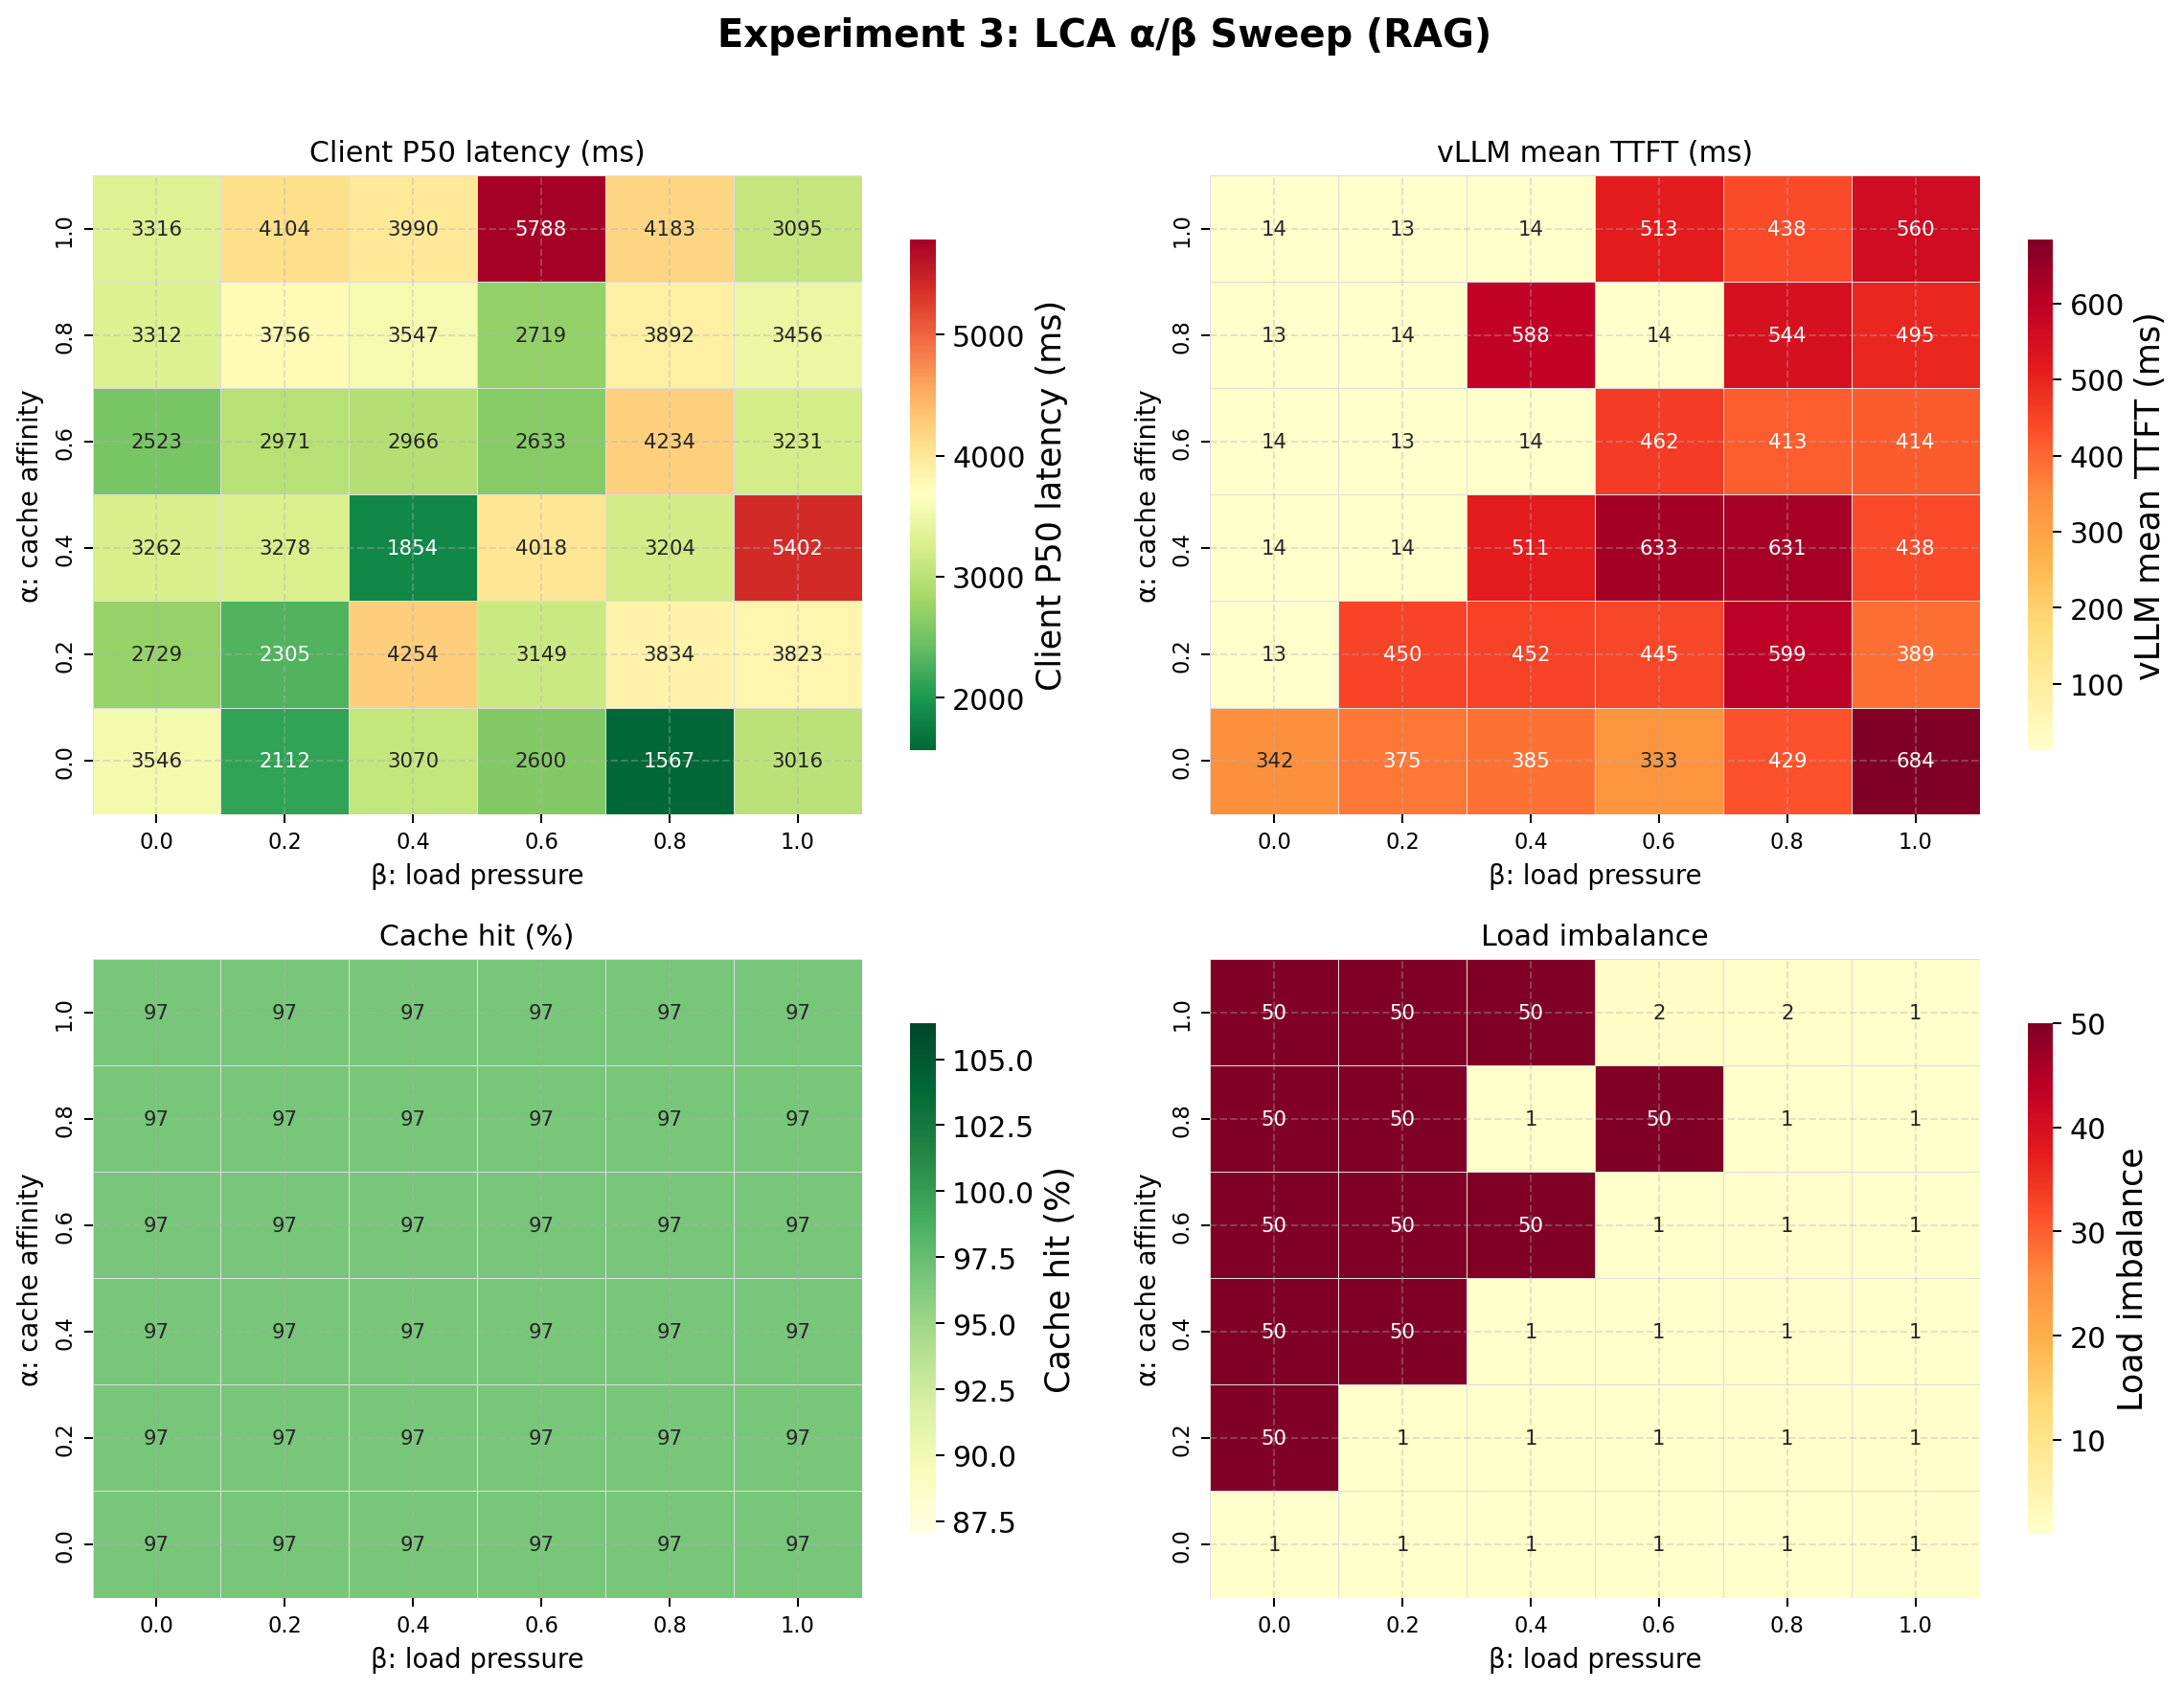
\includegraphics[width=0.95\linewidth]{figures/exp3_rag_heatmaps.png}
    \caption{Experiment~3 RAG sensitivity sweep. Cache hit rate remains flat because the shared system prompt is already warmed, while the imbalance heatmap exposes cache-heavy settings that collapse traffic onto one backend.}
    \label{fig:exp3_rag_heatmap}
\end{figure}

Figure~\ref{fig:exp3_sharegpt_heatmap} shows the same sweep on ShareGPT. Unlike RAG, ShareGPT does not saturate prefix-cache hit rate. Cache hit rates range from roughly 36\% to 47\%, making the sweep more informative about the locality side of the tradeoff. However, latency remains noisy because the two instances contend for the same GPU.

\begin{figure}[H]
    \centering
    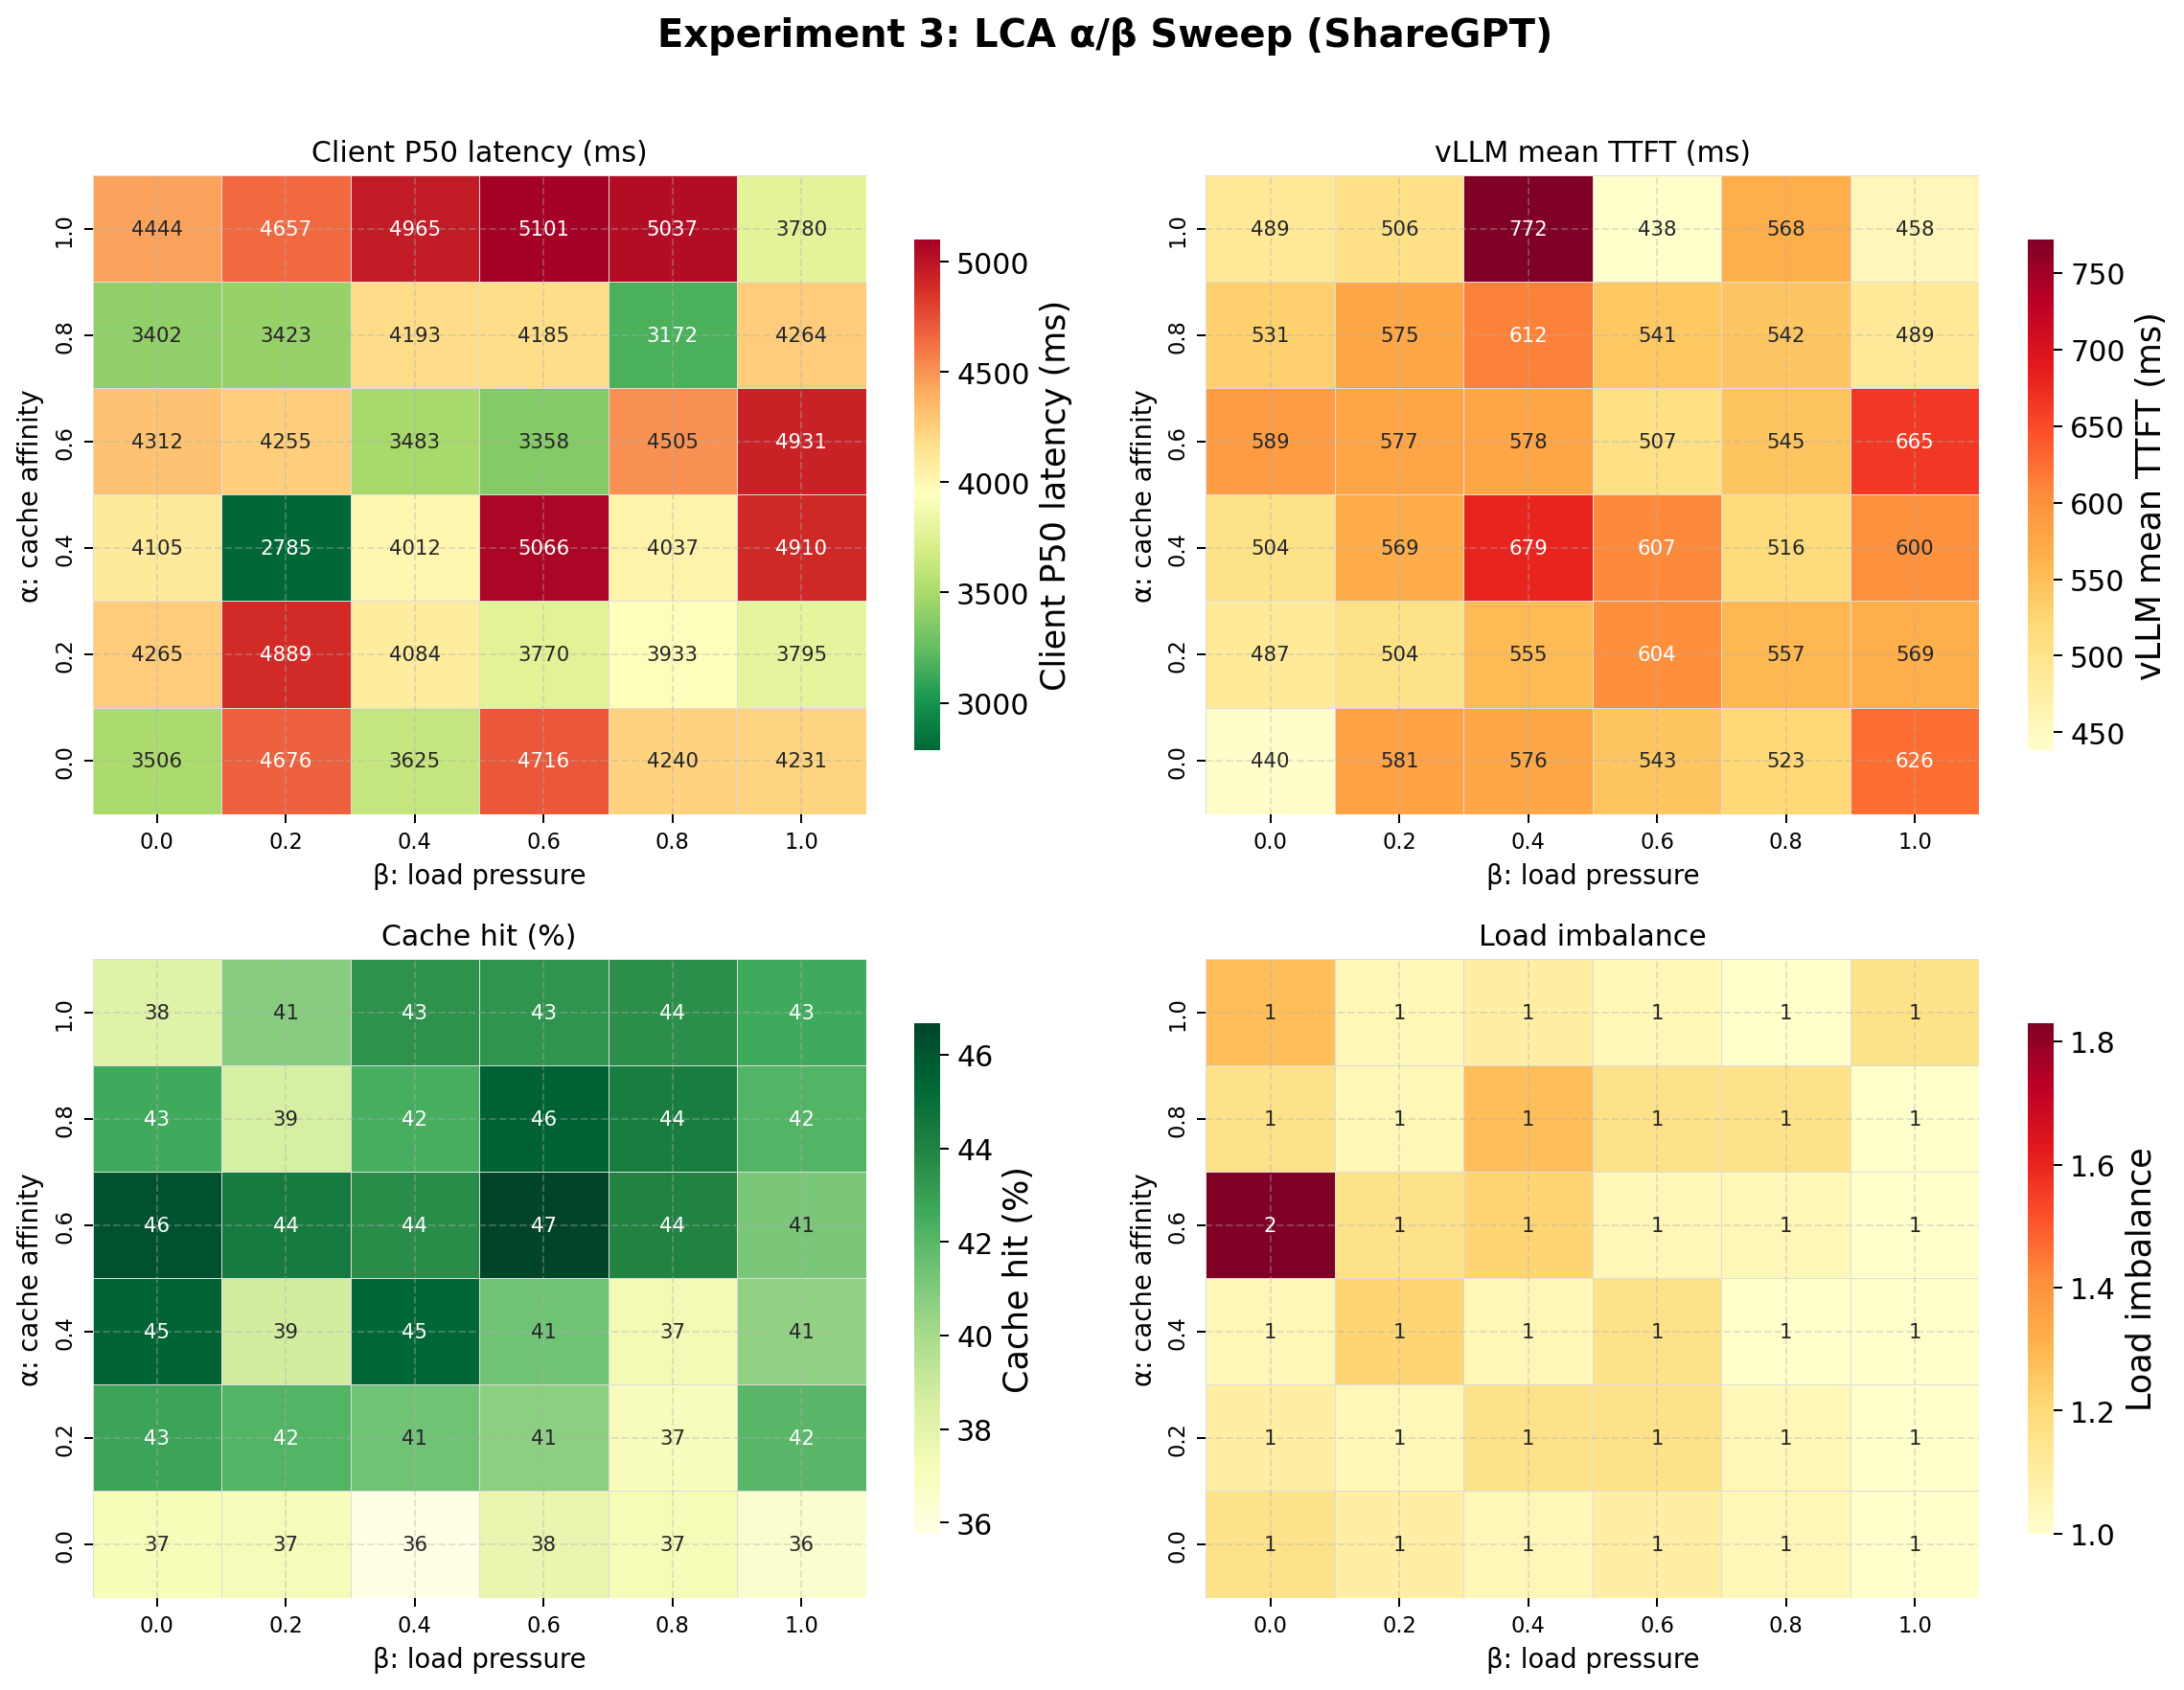
\includegraphics[width=0.95\linewidth]{figures/exp3_sharegpt_heatmaps.png}
    \caption{Experiment~3 ShareGPT sensitivity sweep. ShareGPT exposes a more meaningful cache-hit range than RAG, but the shared-GPU setup still makes absolute latency noisy.}
    \label{fig:exp3_sharegpt_heatmap}
\end{figure}

\begin{table}[H]
    \caption{Best balanced LCA settings from Experiment~3 using imbalance $\leq 1.3$. These are candidate regions, not universal defaults.}
    \label{tab:exp3_best}
    \centering
    \small
    \begin{tabular}{@{}lccrrrr@{}}
        \toprule
        \textbf{Workload} & $\boldsymbol{\alpha}$ & $\boldsymbol{\beta}$ & \textbf{P50 Lat.} & \textbf{P95 Lat.} & \textbf{Cache Hit} & \textbf{Imbal.} \\
        \midrule
        RAG      & 0.0 & 0.8 & 1566.7 & 2851.0  & 96.7 & 1.00 \\
        RAG      & 0.4 & 0.4 & 1854.3 & 3299.8  & 96.7 & 1.00 \\
        RAG      & 0.2 & 0.2 & 2305.3 & 3760.5  & 96.7 & 1.08 \\
        ShareGPT & 0.4 & 0.2 & 2785.4 & 4046.6  & 38.7 & 1.22 \\
        ShareGPT & 0.8 & 0.8 & 3171.9 & 7613.0  & 44.3 & 1.16 \\
        ShareGPT & 0.6 & 0.6 & 3357.7 & 10125.6 & 46.7 & 1.05 \\
        \bottomrule
    \end{tabular}
\end{table}

\begin{figure}[H]
    \centering
    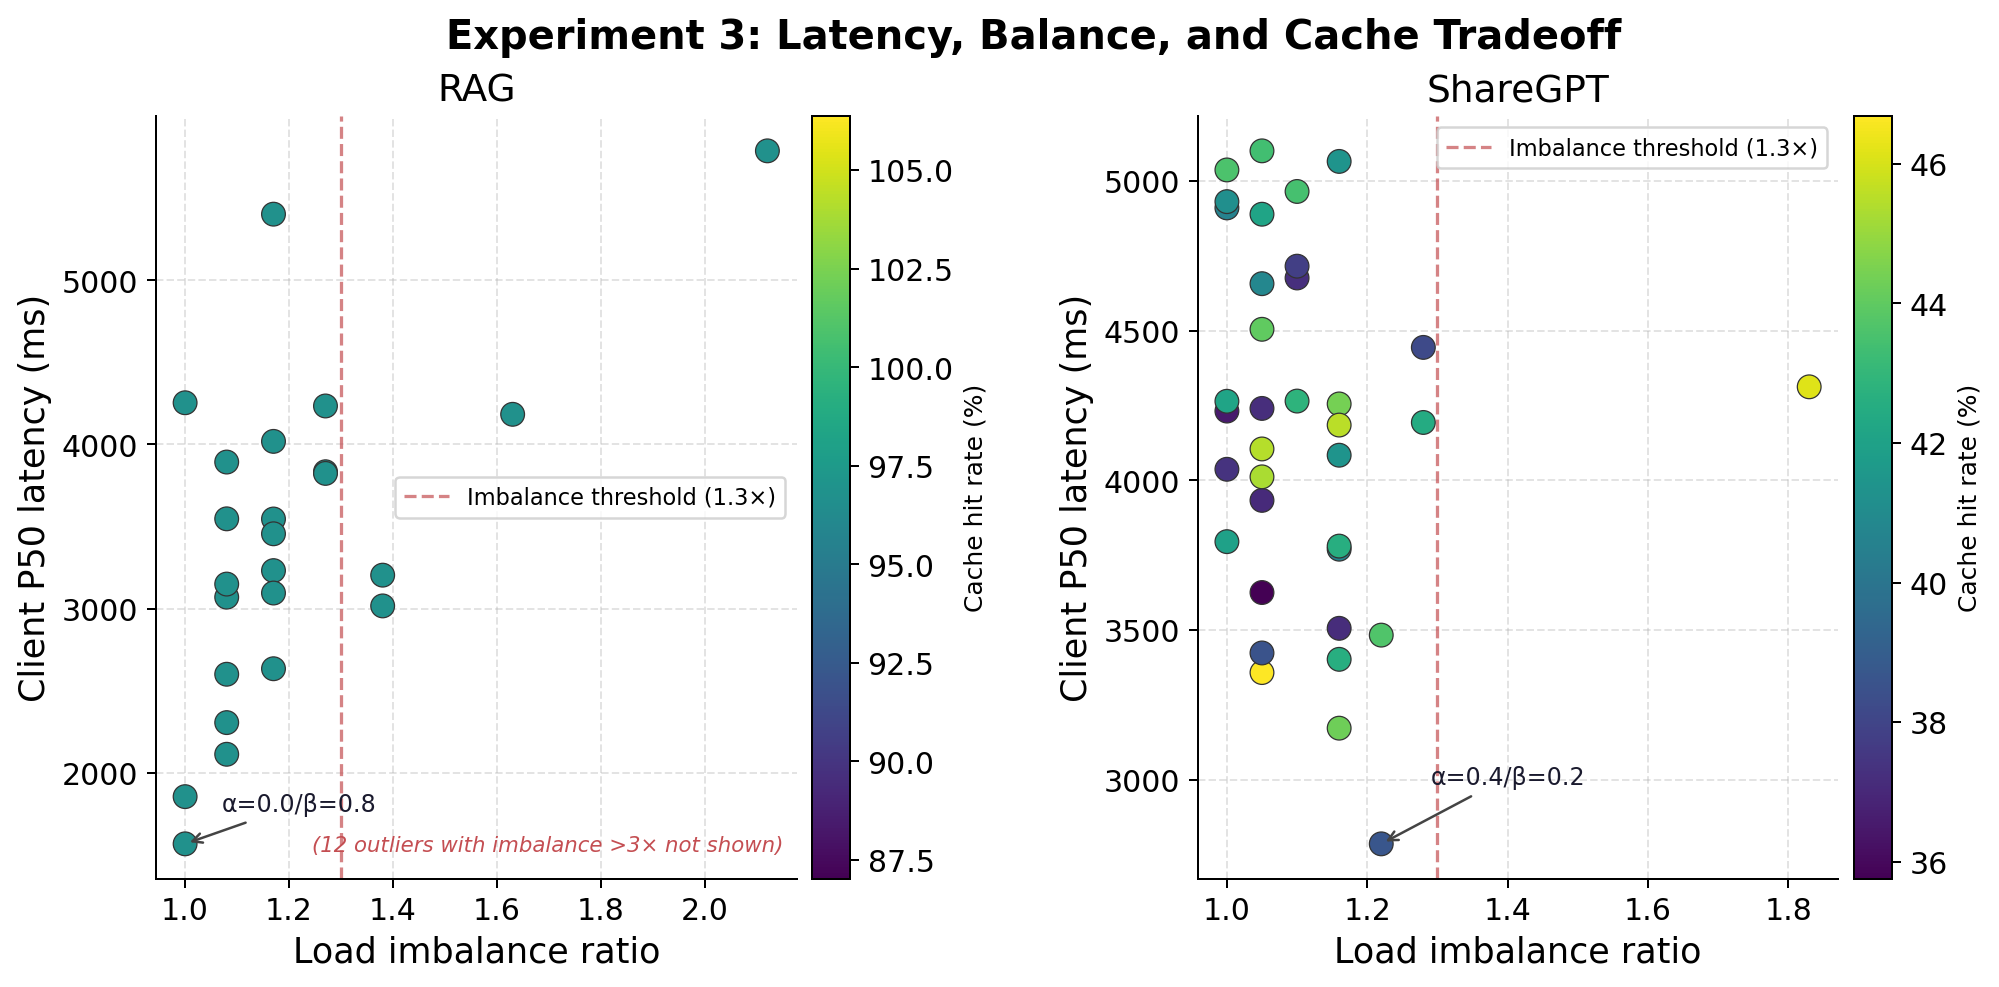
\includegraphics[width=0.95\linewidth]{figures/exp3_lca_tradeoff.png}
    \caption{Latency, balance, and cache tradeoff for the LCA sweep. The dashed line marks imbalance 1.3. The RAG workload shows catastrophic imbalance for several cache-heavy settings; ShareGPT remains more balanced but has a noisier latency/cache frontier.}
    \label{fig:exp3_tradeoff}
\end{figure}

\paragraph{Summary of completed experiments.}
The combined results support three conservative claims. First, routing affects cache reuse on workloads with reusable prefixes, especially multi-turn chat. Second, a shared-prefix RAG workload can make cache hit rate uninformative because all policies eventually reuse the same system prompt. Third, LCA requires workload-aware tuning: cache affinity must be counterbalanced by running-load and in-flight pressure, or the policy can over-concentrate traffic.

\subsection{Experiment 4: cache directory staleness}
\label{sec:eval_staleness}

The cache-directory staleness sweep remains future work. The implemented experiment varies the directory staleness parameter $\delta \in \{0, 0.1, 0.5, 1.0, 5.0, 30.0\}$ seconds under LCA. This will test how long proxy-side cache-affinity entries can remain useful before eviction or workload drift makes them misleading.

% ===========================================================================
% 6. RELATED WORK
% ===========================================================================
\section{Related work}
\label{sec:related}

\paragraph{Single-node KV cache management.}
vLLM~\citep{kwon2023pagedattention} introduced PagedAttention, which uses OS-style virtual memory paging for KV cache blocks, enabling near-zero memory waste and efficient sharing. SGLang~\citep{zheng2024sglang} further improves prefix sharing with RadixAttention, using a radix tree structure for automatic prefix reuse. CachedAttention~\citep{gao2024cachedattention} extends cache reuse across multi-turn conversations by persisting KV cache entries between requests. LayerKV~\citep{xiong2024layerkv} identifies that TTFT degradation is driven by KV cache allocation queuing and proposes layer-wise management. Li et al.~\citep{li2024kvcache_survey} provide a comprehensive survey of KV cache optimization techniques across token, model, and system levels. These works optimize cache management \emph{within} a single instance; we study routing \emph{across} instances.

\paragraph{Distributed scheduling for LLM serving.}
Preble~\citep{tao2024preble} implements cache-aware prompt scheduling by tracking cached prefixes across instances, similar to our approach but integrated into a custom scheduler. DualMap~\citep{zhu2025dualmap} uses two mapping layers---a cache affinity map and a load balance map---to achieve both goals simultaneously. Mooncake~\citep{qin2025mooncake} disaggregates KV cache from compute into a distributed pool, enabling cross-instance cache sharing. KVShare~\citep{yang2025kvshare} enables multi-tenant KV cache reuse within a single instance, achieving up to 9.39$\times$ TTFT reduction. These systems require engine modifications or custom schedulers; our approach operates at the gateway level with unmodified vLLM instances.

\paragraph{Phase disaggregation.}
Splitwise~\citep{patel2024splitwise} and DistServe~\citep{zhong2024distserve} separate prefill and decode phases onto different hardware pools, optimizing each independently. Sarathi-Serve~\citep{agrawal2024sarathi} introduces chunked-prefill scheduling to reduce decode latency interference. These approaches address prefill cost through hardware specialization; we address it through cache-aware routing.

\paragraph{Classic load balancing.}
Consistent hashing~\citep{karger1997consistent} provides session affinity with minimal redistribution on topology changes. The power-of-two-choices~\citep{mitzenmacher2001power} achieves exponential tail improvement with minimal information. We include both as baselines and extend them with cache-aware dimensions. Ray Serve's PrefixCacheAffinityRouter~\citep{rayserve2024prefix} is a recent industry implementation of prefix-aware routing within the Ray ecosystem.

\paragraph{Theoretical foundations.}
Jaillet et al.~\citep{jaillet2026online_scheduling} model LLM scheduling with KV cache constraints as an online optimization problem, proving that no deterministic online algorithm achieves a constant competitive ratio under adversarial arrivals. This theoretical result justifies our empirical approach using heuristic scoring policies.

% ===========================================================================
% 7. DISCUSSION & LIMITATIONS
% ===========================================================================
\section{Discussion and limitations}
\label{sec:discussion}

\paragraph{When does cache-aware routing matter?}
Our results suggest that cache-aware routing provides the most benefit when: (1) prefixes are \emph{long}, making cache miss costly; (2) \emph{prefix reuse is high}, as in multi-turn conversations or shared system prompts; and (3) the number of instances $N$ exceeds the number of distinct prefix groups, creating routing ambiguity. For short, single-turn requests with unique prompts, all policies converge because cache hits are rare regardless.

\paragraph{Practical recommendation.}
For deployments with multi-turn or shared-prefix workloads, we recommend using cache-aware routing only with explicit load-pressure terms that include waiting, running, and router-side in-flight requests. The current measurements do \emph{not} justify a universal $\alpha/\beta$ default. Instead, the sweep suggests choosing workload-specific settings and rejecting configurations that achieve low TTFT by collapsing traffic onto one backend. The simplicity of the scoring function ($O(N)$ per request) introduces negligible overhead, but the weights must be validated under the target workload.

\paragraph{Limitations.}
Several limitations should be noted:
\begin{itemize}
    \item \textbf{Single GPU, two instances.} Our testbed shares one RTX~5080 between two vLLM instances, introducing GPU contention absent in production deployments. All reported metrics are relative comparisons; absolute numbers should not be generalized.
    \item \textbf{Small model.} We use Qwen2.5-0.5B-Instruct, which has shorter prefill times than production-scale models. Cache-aware routing benefits are likely \emph{larger} with bigger models where prefill is more expensive.
    \item \textbf{Two instances.} With $N = 2$, the routing problem is simpler than at scale. We plan to validate with a trace-driven simulator at $N = 4, 8, 16$.
    \item \textbf{Proxy-side cache directory.} Our Option~C directory infers cache state from routing history, which can become inaccurate after cache eviction. A direct query of vLLM's cache state would improve accuracy.
    \item \textbf{Limited workload diversity.} We primarily evaluate on ShareGPT multi-turn conversations. Different workloads (e.g., code completion, long-document QA) may exhibit different prefix-sharing patterns.
\end{itemize}

% ===========================================================================
% 8. BROADER IMPACT
% ===========================================================================
\section{Broader impact}
\label{sec:impact}

\paragraph{Energy efficiency.} Cache-aware routing can reduce redundant KV cache computation, directly saving GPU cycles when prefixes are long and reused. In the ShareGPT experiment, cache-aware policies reduce cache misses by approximately 30 percentage points relative to round-robin. At deployment scale, reducing unnecessary prefill work could contribute to the Green AI agenda by lowering the per-request energy footprint of LLM inference.

\paragraph{Fairness.} Cache-aware routing can create ``hot'' instances where users whose sessions map to less-loaded instances receive faster responses. The LCA scoring policy mitigates this by incorporating load pressure, but practitioners should monitor per-instance tail latencies and consider fairness-aware extensions.

% ===========================================================================
% 9. CONCLUSION
% ===========================================================================
\section{Conclusion}
\label{sec:conclusion}

We presented a systematic evaluation of six gateway-level routing policies for multi-instance LLM serving with prefix caching. Using ground-truth metrics from vLLM's Prometheus endpoint, we demonstrated that:
\begin{itemize}
    \item Cache-aware routing improves cache hit rates on multi-turn chat, from 68\% under round-robin to roughly 98\% under affinity-based policies.
    \item Pure affinity can create load imbalance, and the same risk appears more sharply in the RAG workload where cache-heavy LCA collapses all traffic onto one backend.
    \item RAG cache-hit rate is not sufficient evidence of routing quality: a single shared system prompt saturates cache reuse across all policies, so load balance and client-observed latency must be reported alongside TTFT.
    \item The LCA scoring function is useful as a tunable mechanism, but the $\alpha/\beta$ setting must be validated per workload rather than treated as a fixed default.
\end{itemize}

Our results provide practical guidance for deploying LLM serving gateways: use cache-aware routing when prefix reuse is expected, measure load imbalance as a first-class metric, and tune cache affinity against live load pressure before making claims about latency improvements. All code, experiment configurations, and analysis artifacts are released for reproducibility.

% ===========================================================================
% ACKNOWLEDGMENTS
% ===========================================================================
\begin{ack}
This work was completed as part of the COSC~6375 Graduate Research course at the University of Texas Permian Basin. We thank the course instructors for providing the project framework and evaluation criteria. AI coding assistants (GitHub Copilot, Claude, Gemini) were used for code implementation support; all experimental design, result interpretation, and writing represent the author's own intellectual contributions. The experimental hardware was a personal NVIDIA RTX~5080 GPU.
\end{ack}

% ===========================================================================
% REFERENCES
% ===========================================================================
\bibliographystyle{plainnat}
\bibliography{references}

% ===========================================================================
% APPENDIX
% ===========================================================================
\appendix

\section{Detailed per-trial results}
\label{app:per_trial}

Table~\ref{tab:per_trial} provides full per-trial breakdowns for Experiment~1. Each trial uses a different random seed for workload generation, with all policies receiving identical request sequences within a trial.

\begin{table}[h]
    \caption{Per-trial results for Experiment~1 (ShareGPT multi-turn chat). Each row is one trial (fixed seed), one policy. TTFT and cache hit rate from vLLM Prometheus metrics.}
    \label{tab:per_trial}
    \centering
    \small
    \begin{tabular}{@{}llccccc@{}}
        \toprule
        \textbf{Policy} & \textbf{Trial} & \textbf{Requests} & \textbf{TTFT (ms)} & \textbf{Cache Hit (\%)} & \textbf{Imbalance} & \textbf{P95 (ms)} \\
        \midrule
        Round-Robin     & 0 & 144 & 550.5 & 70.8 & 1.00 & 3065 \\
        Round-Robin     & 1 & 155 & 1030.2 & 66.1 & 1.01 & 3023 \\
        Round-Robin     & 2 & 158 & 830.3 & 66.8 & 1.00 & 3134 \\
        \midrule
        JSQ             & 0 & 144 & 713.3 & 94.3 & 1.03 & 3093 \\
        JSQ             & 1 & 155 & 806.7 & 93.8 & 1.09 & 3137 \\
        JSQ             & 2 & 158 & 833.5 & 94.3 & 1.03 & 3134 \\
        \midrule
        P2C             & 0 & 144 & 1045.7 & 96.4 & 1.15 & 3147 \\
        P2C             & 1 & 155 & 704.6 & 97.4 & 1.21 & 3124 \\
        P2C             & 2 & 158 & 966.5 & 98.3 & 1.08 & 3129 \\
        \midrule
        Session Aff.    & 0 & 144 & 918.5 & 98.8 & 1.57 & 3084 \\
        Session Aff.    & 1 & 155 & 738.0 & 98.0 & 1.31 & 3144 \\
        Session Aff.    & 2 & 158 & 930.8 & 98.7 & 1.55 & 3083 \\
        \midrule
        Prefix-Key Aff. & 0 & 144 & 870.9 & 98.2 & 1.72 & 3125 \\
        Prefix-Key Aff. & 1 & 155 & 744.7 & 98.6 & 1.12 & 3104 \\
        Prefix-Key Aff. & 2 & 158 & 855.7 & 98.3 & 1.23 & 3124 \\
        \midrule
        Load+Cache (LCA) & 0 & 144 & 887.3 & 97.1 & 1.44 & 3234 \\
        Load+Cache (LCA) & 1 & 155 & 1203.8 & 98.9 & 1.18 & 3181 \\
        Load+Cache (LCA) & 2 & 158 & 869.4 & 98.8 & 1.00 & 3249 \\
        \bottomrule
    \end{tabular}
\end{table}

\section{Implementation details}
\label{app:implementation}

\paragraph{Software stack.} The router is implemented in Python using FastAPI (HTTP server), LangGraph (pipeline orchestration), and \texttt{aiohttp} (async HTTP client for backend forwarding and metrics scraping). Policy selection is controlled via the \texttt{ROUTING\_POLICY} environment variable. The total router codebase is approximately 500 lines of Python.

\paragraph{Experiment runner.} Automated experiment sweeps are managed by an 828-line Python script (\texttt{run\_experiments.py}) that handles router lifecycle management (start/stop per policy), open-loop load generation with \texttt{asyncio}, vLLM metrics snapshot differencing, and multi-trial execution with fixed seeds.

\paragraph{Reproducibility.} All experiments use fixed random seeds (42, 123, 7) for workload generation. The experiment runner saves JSON summaries and JSONL raw logs per trial. Complete instructions and launch commands are documented in the repository README.

\paragraph{LLM usage disclosure.} AI coding assistants were used for implementation support and editing assistance. The experimental methodology, result interpretation, and claims are the author's own work.

% ===========================================================================
% NEURIPS PAPER CHECKLIST
% ===========================================================================
\newpage
\input{checklist}

\end{document}
